\universidade{Universidade de São Paulo \\ Instituto de Física de São Carlos}

\autor{Autor da tese}

\titulo{T\'{\i}tulo da sua tese}

\orientador{Prof. Dr. Nome do Seu Orientador}

\area{Física Básica}

\comentario{Dissertação apresentada ao Programa de Pós-Graduação em Física do Instituto de Física de São Carlos da Universidade de São Paulo, para obtenção do título de mestre em Ciências.}

\instituicao{Grupo de Pesquisa \par Departamento Disso ou Daquilo \par Instituto de Física de São Carlos - Universidade de São Paulo}

\local{São Carlos}

\data{2011}

\capa

\folhaderosto

\begin{center}
  {\scshape \ttfamily AUTORIZO A REPRODUÇÃO E DIVULGAÇÃO TOTAL OU PARCIAL DESTE TRABALHO, POR QUALQUER MEIO CONVENCIONAL OU ELETRÔNICO, PARA FINS DE ESTUDO E PESQUISA, DESDE QUE CITADA A FONTE.}
  
  \vfill
  
  \begin{center}
    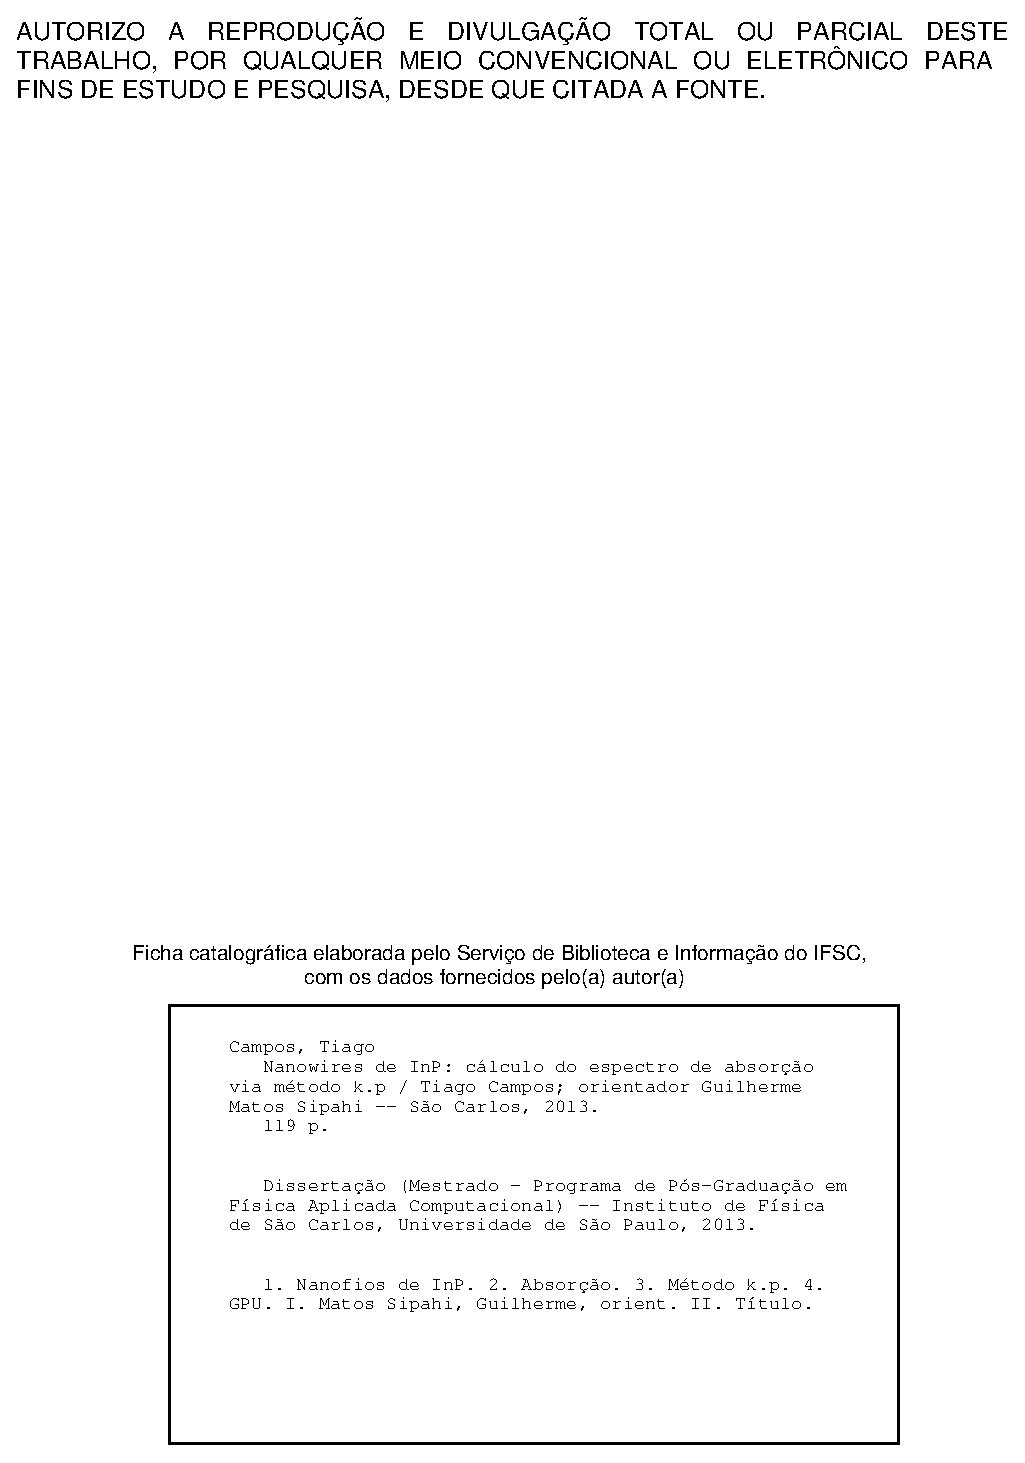
\includegraphics[scale = 0.28]{fichacatalografica}
  \end{center}
\end{center}


% \begin{folhadeaprovacao}
% Dissertação apresentada ao Programa de Pós-Graduação em Física do Instituto de Física de São Carlos da Universidade de São Paulo, para obtenção do título de mestre em Ciências.
% 
% \assinatura{Prof. Dr. Esmerindo de Sousa Bernardes\\ Orientador}  
% \assinatura{Prof. Dr. Iouri Poussep\\ Instituto de Física de São Carlos -- Universidade de São Paulo}
% \assinatura{Prof. Dr. Marcel Novaes\\ Departamento de Física -- Universidade Federal de São Carlos}
% \end{folhadeaprovacao}